\section{Référence de la classe CDOMElement}
\label{class_c_d_o_m_element}\index{CDOMElement@{CDOMElement}}
Graphe d'héritage de CDOMElement::\begin{figure}[H]
\begin{center}
\leavevmode
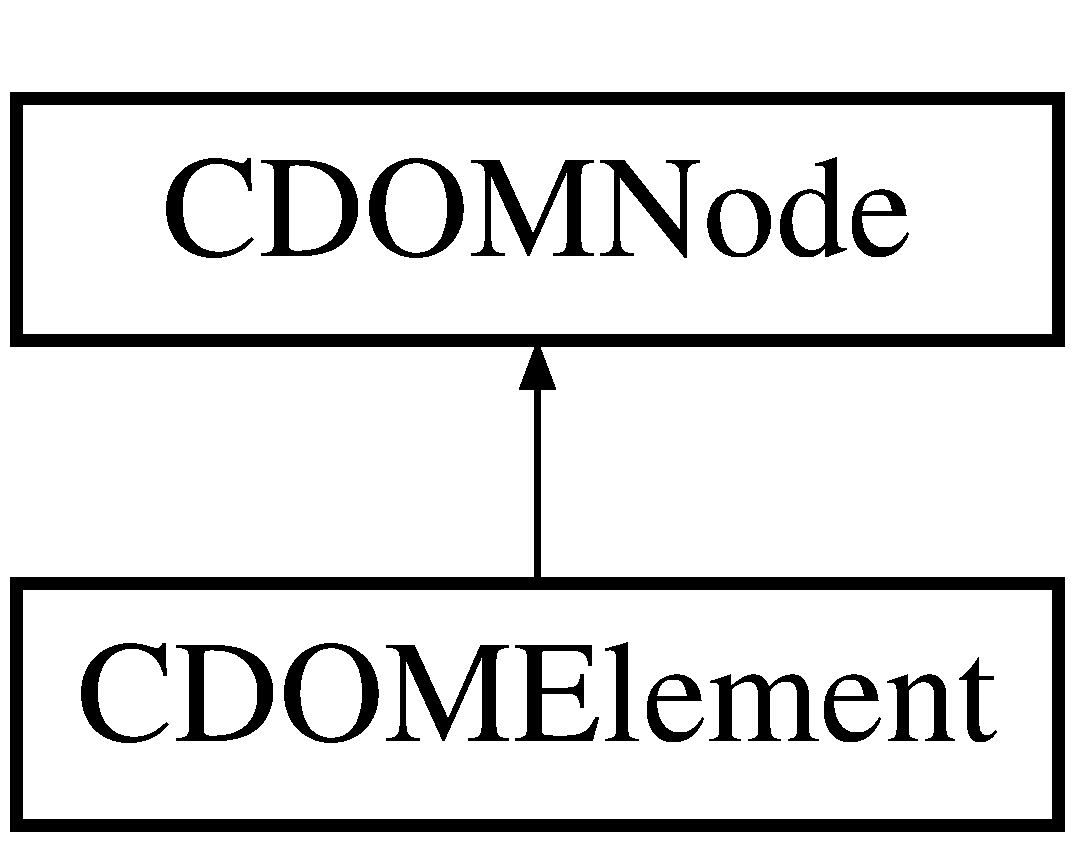
\includegraphics[height=2cm]{class_c_d_o_m_element}
\end{center}
\end{figure}


\subsection{Description détaillée}
Classe reproduisant en PHP 4 le comportement de la classe {\tt DOMElement} de la bibliothèque DOM PHP 5. \subsection*{Fonctions membres publiques}
\begin{CompactItemize}
\item 
{\bf CDOMElement} (\$name, \$value=NULL, \$namespaceURI=NULL)
\begin{CompactList}\small\item\em Constructeur. \item\end{CompactList}\item 
{\bf setAttribute} (\$name, \$value)
\begin{CompactList}\small\item\em Assigne une valeur à un attribut de l'élément. \item\end{CompactList}\end{CompactItemize}


\subsection{Documentation des fonctions membres}
\index{CDOMElement@{CDOMElement}!CDOMElement@{CDOMElement}}
\index{CDOMElement@{CDOMElement}!CDOMElement@{CDOMElement}}
\subsubsection{\setlength{\rightskip}{0pt plus 5cm}CDOMElement::CDOMElement (\$ {\em name}, \/  \$ {\em value} = {\tt NULL}, \/  \$ {\em namespaceURI} = {\tt NULL})}\label{class_c_d_o_m_element_83adcf60034e908baeb6cd1a42826f31}


Constructeur. 

Crée un élément DOM

\begin{Desc}
\item[Paramètres:]
\begin{description}
\item[{\em name}]le nom de l'élément à créer \item[{\em value}]la valeur à attribuer à l'élément (A TESTER) \item[{\em namespaceURI}]l'URI d'un espace de nom pour créer l'élément dans un espace de nom spécifique (INCOMPLET)\end{description}
\end{Desc}
\begin{Desc}
\item[{\bf À faire}]L'attribution immédiate d'une valeur utilise la méthode {\tt setContent()} des objets DOM PHP4, cela semble fonctionner pour créer des éléments XML (balises) avec un contenu texte, mais je ne sais pas si d'autres utilisations sont possibles\end{Desc}
\begin{Desc}
\item[{\bf À faire}]Pour l'instant la création dans un espace de nom (3è paramètre) n'est pas implémentée \end{Desc}
\index{CDOMElement@{CDOMElement}!setAttribute@{setAttribute}}
\index{setAttribute@{setAttribute}!CDOMElement@{CDOMElement}}
\subsubsection{\setlength{\rightskip}{0pt plus 5cm}CDOMElement::setAttribute (\$ {\em name}, \/  \$ {\em value})}\label{class_c_d_o_m_element_4b57f1fd3690eea06761b009c9c0a1d5}


Assigne une valeur à un attribut de l'élément. 

Si l'attribut n'existe pas, il est créé

\begin{Desc}
\item[Paramètres:]
\begin{description}
\item[{\em name}]le nom de l'attribut auquel on veut assigner une valeur \item[{\em value}]la valeur à assigner à l'attribut\end{description}
\end{Desc}
\begin{Desc}
\item[Renvoie:]l'ancien objet DomAttribute si l'attribut avait déjà une valeur, sinon le nouvel objet (INCOMPATIBLE)\end{Desc}
\begin{Desc}
\item[{\bf À faire}]La valeur de retour (un objet DomAttribute) n'est pas la même que pour le \char`\"{}vrai\char`\"{} DOM PHP 5 qui, d'après la doc PHP, retourne TRUE ou FALSE. A tester \end{Desc}


La documentation de cette classe a été générée à partir du fichier suivant :\begin{CompactItemize}
\item 
src/lib/dom/{\bf dom-php4.class.php}\end{CompactItemize}
